\section{Farmaci del sistema cardiovascolare e renale}

\subsection{Farmaci anti--ipertensivi}

\begin{tikzpicture}
	\Tree
	[.Anti-ipertensivi diuretici simpaticolitici vasodilatatori ]
\end{tikzpicture}

\begin{tikzpicture}
	\Tree
	[.{Diuretici\\ (capitolo ah hoc)}
		[.{Diuretici dell'ansa} \node[farmaco]{furosemide}; ]
		[.{Inibitori del simporto\\ \ce{Na+}-\ce{Cl-}} \node[farmaco]{tiazidici}; ]
		[. {Risparmiatori di \ce{K+}} \node[farmaco]{spironolattone}; ]
	]
\end{tikzpicture}

\begin{tikzpicture}
	\tikzset{level 3/.style={level distance=120pt}}
	\Tree
	[.Simpaticolitici
		[.{SNC}
			[.\node[farmaco]{$\alpha$-metildopa}; {Inibitore dopa-carbossilasi\\ emergenza ipertensiva \\ Da sedazione, tossicit\`a epatica\\ coombs positivo} ]
			[.\node[farmaco]{clonidina}; {Agonista $\alpha_2$. $\downarrow$noradrenalina\\ Usato in gravidanza \\ Da sonnolenza, depressione\\ $\downarrow$libido, secchezza fauci } ]
		]		
		[.{$\beta$--bloccanti}
			[.\node[farmaco]{propranololo}; {Usato in ipertensione, scompenso cardiaco, \\ aritmie, glaucoma. Produce $\downarrow$GC e renina. \\ Da affaticamento,$\downarrow$umore, insomnia, $\uparrow$glicemia, \\ alterazione assetto lipidico (i non ASI). \\ Interruzione improvvisa $\uparrow$infarto.} ]
		]		
		[.{$\alpha$--agonisti} \node[farmaco]{doxazosina}; ]
		[.{Misti $\alpha$/$\beta$}
			[.\node[farmaco]{labetalolo}; {ipertensione da feocromocitoma.\\ Da prurito intenso, $\downarrow$eiaculazione} ]
		]
	 ]
\end{tikzpicture}

\begin{tikzpicture}
	\tikzset{level distance=80pt, level 4/.style={level distance=100pt}}
	\Tree
	[.{Vasodilatatori}
		[.{diretti}
			[.{prevalentemente\\ arteriosi}
				[.{Inibitori IP3} \node[farmaco]{idralazina\\ (non pi\`u usato)}; ]
				[.{\ce{Ca^{2+}} antagonisti}  \node[farmaco]{nifedipina\footnotemark\\ (anche verapamil\\ e diltiazem\\ ma su cuore)}; ]
			]
			[.{arterovenosi} 
				[.{rilascio \ce{NO}} \node[farmaco]{nitroprussiato\footnotemark\\ nitroglicerina}; ]
			]
		]
		[.{indiretti}
			[.{ACE inibitori}
				[.\node[farmaco]{captopril\\ enalapril\\ fosinopril}; {Dilata arteriole e grandi vene. \\$\downarrow$pre/post carico. \\ Non inficia riflesso barocettivo\\ ne secrezione di aldosterone. \\ $\uparrow$bradichinina da tosse secca\\ e edema angioneurotico.} ]
			]
			[.{Antagonisti AT--1}
				[.{sartani} {Uso in ipertensione, ACC, \\ nefropatia diabetica\\ NO in gravidanza} ]
			]
		]
	]
\end{tikzpicture}

\footnotetext{Vedere farmaci angina}

\footnotetext{Vedere farmaci angina}

\newpage

\subsection{Farmaci nell'angina e infarto cardiaco}

\begin{tikzpicture}
	\Tree
	[.{angina\\ infarto} vasodilatatori simpaticomimetici ]
\end{tikzpicture}

\begin{tikzpicture}
	\tikzset{level distance=90pt, level 3/.style={level distance=130pt}}
	\Tree
	[.{Vasodilatatori}
		[.Nitrati
			[.\node[farmaco]{Isosorbide mononitrato}; {Duranta d'azione pi\`u lunga} ]
			[.\node[farmaco]{Nitroglicerina}; {Rilascio \ce{NO}, $\uparrow$cGMP, relax muscolatura lis.\\ Via sublinguale, transdermica, rapido assorbimento\\ grazie alla solubilit\`a lipidica}  ]	
		]
		[.{\ce{Ca^{2+}}  antagonisti}
			[.\node[farmaco]{verapamil\\ (diidropiridine)}; {$\downarrow$conduzione NSA. $\downarrow$ RVP} ]
			[.\node[farmaco]{diltiazem}; {$\downarrow$conduzione NSA. $\downarrow$ RVP} ]
			[.\node[farmaco]{nifedipina}; {$\updownarrow$conduzione NSA.  Possibile tachicardia riflessa\\ minori effetti cardiaci} ]
		]
	]
\end{tikzpicture}

\begin{tikzpicture}
	\tikzset{level distance=90pt, level 3/.style={level distance=130pt}}
	\Tree
	[.{Simpaticolitici}
		[.{$\beta$--bloccanti}
			[.\node[farmaco]{propranololo\footnotemark}; {$\downarrow$GC, $\downarrow$PA, $\downarrow$consumo \ce{O2} micardico} ]
		]
	]
\end{tikzpicture}

\footnotetext{vedi farmaci anti-ipertensivi}

\begin{tikzpicture}
	\node[chartnode,anchor=west] at(0,0)(mlck){MLCK} node[chartnode,xshift=125pt] (mlckstar){MLCK${}^*$};
	\draw[drawarrow](mlck)[yshift=10pt]--node[smallfont,yshift=6pt,midway](Ca){\ce{Ca^{2+}}}
				node[chartnode,yshift=50pt,midway](CCa){Canali \ce{Ca^{2+}}}
				node[smallfont,yshift=-15pt,midway](camp){cAMP}
				node[chartnode,yshift=-60pt,midway](atp){ATP}(mlckstar);
	\draw[drawarrow] (mlckstar) [yshift=-10pt] -- (mlck);
	\draw[drawarrow] (CCa)-- node[midway](CCCa){} node[smallfont,xshift=5em](bloc){bloccanti canali} (Ca);
	\draw[drawarrow] (bloc)-- node[midway, below]{$\ominus$} (CCCa);
	\draw[drawarrow] (atp)-- node[midway](catp){} node[smallfont,xshift=5em](beta){$\beta$-bloccanti} (camp);
	\draw[drawarrow] (beta)-- node[midway, above]{$\oplus$} (catp);
	
	\node[chartnode,below right=1em and 2em of mlckstar](mlc){MLC};
	\node[chartnode,right=50pt of mlc](mlcstar){MLC${}^*$} node[right=3pt of mlcstar](+){+}
		node[chartnode, right=3pt of +](actina){actina};
	\node[chartnode,above=20pt of actina](contrazione){contrazione};
	\node[chartnode,below=20pt of mlc](relax){relax};
	\draw[drawarrow] (mlc) [yshift=10pt]-- node[midway](a){}(mlcstar);
	\draw[drawarrow] (mlcstar) [yshift=-10pt]-- 
		node[smallfont,midway,yshift=-6pt](cgmp){cGMP} 
		node[chartnode,yshift=-57pt,midway](gtp){GTP}
		(mlc);
	\draw[drawarrow] (actina) -- (contrazione);
	\draw[drawarrow] (mlc) -- (relax);
	\draw[drawarrow] (mlckstar) -| (a);
	\draw[drawarrow] (gtp)-- node[midway](cgtp){} 
		node[smallfont,xshift=10pt](gcstar){GC${}^*$}
		node[chartnode,xshift=100pt](gc){Guanil ciclasi} 
		(cgmp);
	\draw[drawarrow] (gc)-- node[midway](cgc){} node[midway, chartnode,yshift=-50pt](no){NO} (gcstar);
	\draw[drawarrow] (no)--node[midway, right]{$\oplus$}(cgc);
	
	\node[smallfont,text width=12em,anchor=west] at(0,-4) {* $\equiv$ elemento attivato\\
	MLCK $\equiv$ Miosina Catena Leggera chinasi\\ MLC $\equiv$ Miosina Catena Leggera};
\end{tikzpicture}

\begin{tikzpicture}
	\Tree
	[.Angina 
		[.{ischemia cardiaca transitoria\\ senza danno al miocardio}
			{stabile}
			{instabile}
			{di prinzmetal}
			{silente}
			{cronica}
		]
	]		
\end{tikzpicture}

\begin{tikzpicture}
	\Tree
	[.Terapia
		comportamentale
		chirurgica
		[.farmacologica
			[.{vasodilatatori\\ \ce{NO} e \ce{Ca^{2+}} antagonisti}
				{per aumentare il flusso}
			]
			[.antiaggreganti {per evitare i trombi}
			]
			[.fibrinolitici {per distruggere i\\ trombi preesistenti}
			]
			[.{$\beta$--bloccanti} {per ridurre il fabbisogno energetico}
			]
			[.oppioidi {per ridurre il dolore}
			]
		]
	]
\end{tikzpicture}

\begin{tikzpicture}
	\Tree
	[.terapia
		[.stabile
			{nitrati organici}
			{$\beta$--bloccanti}
			{statina}
			{aspirina}
		]
		[.instabile
			{nitrati}
			{aspirina}
			{eparina}
		]
		[.variante
			{nitrati organici}
			{\ce{Ca^{2+}} antagonisti}
		]
	]	
\end{tikzpicture}

\subsubsection{Nitrati organici}

\begin{tikzpicture}
	\Tree
	[.{nitrati organici}
		{nitroglicerina}
		{isosorbide mononitrato}
	]
\end{tikzpicture}

\begin{tikzpicture}
	\Tree
	[.effetti
		[.{diminuzione della richiesta\\ di O${}_2$}
			{$\downarrow$ritorno venoso}
			{$\downarrow$volume intracardiaco}
			{$\downarrow$pressione arteriosa}
		]
		[.{scompasa spasmo arterioso} {vasodilatazione arterie\\ coronariche}
		]
	]
\end{tikzpicture}

\begin{tikzpicture}
	\Tree
	[.{effetti collaterali}
		{tachicardia riflessa}
		{aumento riflesso contrattile}
		{riduzione del tempo di perfusione\\ diastolica indotta da tachicardia}
	]
\end{tikzpicture}

\subsubsection{Calcio antagonisti}

\begin{tikzpicture}
	\Tree
	[.tipo
		[.L
			[.{Corrente lunga}
				[.Verapamil
					{cuore}
					{muscolo scheletrico\\ e liscio}
					{neuroni}
					{ossa}
				]
			]
		]
		[.T
			[.{Corrente breve}
				[.Flunarizina
					{cuore}
					{neuroni}
				]
			]
		]
		[.N
			[.{Corrente breve} {neuroni} 
			]
		]
		[.P
			[.{Corrente lunga} {neuroni} 
			]
		]
		[.{Q/R}
			[.{Segnapassi} {neuroni} 
			]
		]
	]
\end{tikzpicture}

\begin{tikzpicture}
	\tikzset{level 2/.style={level distance=120pt}}
	\tikzset{frontier/.style={distance from root=350pt}}
	\Tree
	[.effetti
		[.{muscolo liscio}
			[.{arteriole + sensibili delle venule.\\ Quindi meno effetto di ipotensione ortostatica}
				\node[farmaco]{nifedipina};
			]
		]
		[.{miocardio}
			\node[farmaco]{varapamil\\ diltiazem};
		]
		[.{muscolo scheletrico}
			[.{nessun effetto\\ il \ce{Ca^{2+}} \`e intracellulare} ]
		]
	]
\end{tikzpicture}

\subsubsection{$\beta$--bloccanti}

\begin{tikzpicture}
	\Tree
	[.effetti
		{$\downarrow$frequenza cardiaca}
		{$\downarrow$pressione arteriosa}
		{$\downarrow$contrattilit\`a}
	]
\end{tikzpicture}

\begin{tikzpicture}
	\Tree
	[.{effetti indesiderati}
		{$\uparrow$volume telediastolico}
		{$\uparrow$tempo di eiezione}
		{insomnia}
		{sonni spiacevoli}
		{senso di affaticamento}
		{disfunzione erettile}
	]
\end{tikzpicture}

\begin{tikzpicture}
	\Tree
	[.controindicazioni
		asma
		{affezioni broncospastiche}
		{grave bradicardia}
		{blocco atriventricolare}
		{insufficienza ventricolare sinistra}
	]
\end{tikzpicture}

\subsection{Insufficienza cardiaca}

\begin{tikzpicture}
	\Tree
	[.{I.C.}
		[.{gittata insufficiente\\ a fornire \ce{O2}\\ a organismo}
			[.{i. sistolica}
				{$\downarrow$contrattilità}
				{$\downarrow$fraz. di eiezione}
			]
			[.{i. diastolica}
				{rigidità}
				{perdità di rilasciamento}
			]
		]
	]
\end{tikzpicture}

\begin{tikzpicture}
	\Tree
	[.{scopo del\\ trattamento}
		[.{fase stabile\\(cronica)}
			{$\downarrow$sintomi}
			{rallentare progressione}
		]
		[.{fase scompensata\\(acuta)}
			{ricondurre il paziente\\ alla fare stabile}
		]
	]
\end{tikzpicture}

\begin{tikzpicture}
	\tikzset{level 2/.style={level distance=150pt}}
	\Tree
	[.terapia
		[.{fase cronica}
			{antagonisti aldosterone}
			{ACE inibitori}
			{sartani}
			{$\beta$--bloccanti}
			{digitalici}
			\node(diuretici){diuretici};
			\node(vasodilatatori){vasodilatatori};
		]
		[.\node(acuta){fase acuta};
			{$\beta$--agonisti}
		]
	]
	\draw[drawarrow] (acuta) to[out=0,in=180] (diuretici);
	\draw[drawarrow] (acuta) to[out=0,in=180] (vasodilatatori);
\end{tikzpicture}

\begin{tikzpicture}
	\tikzset{level distance=80pt}
	\Tree
	[.\node(git){$\downarrow$gittata cardiaca};
		[.{$\downarrow$P.A.}
			[.{attivazione barocettori}
				[.\node(simpatico){$\uparrow$simpatico};
					[.{inotropo+} {rimodellamento}
					]
					[.{cronotopo+}
					]
				]
			]
		]
		[.{$\downarrow$flusso renale}
			[.{$\uparrow$renina}
				[.{$\uparrow$angII}
					\node(pre){$\uparrow$ pre--carico};
					[.\node(post){$\uparrow$post--carico};
						\node(fraz){$\downarrow$fraz. eiezione};
					]
				]
			]
		]
	]
	\draw[drawarrow] (simpatico) to[out=0,in=180] (post);
	\draw[drawarrow] (simpatico) to[out=0,in=180] (pre);
	\node[below=1em of fraz](a){};
	\draw[drawarrow] (fraz) --  (a.north) -| (git);
\end{tikzpicture}

\begin{tikzpicture}
	\tikzset{level distance=120pt}
	\Tree
	[.{rimodellamento causato da\\ ipertrofia per riattivazione\\ fattori di crescita}
		[.concentrico
			{da sovraccarico pressorio per \upa post--carico}
		]
		[.eccentrico
			{da sovraccarico volume per \upa pre--carico}
		]
		[.compensato {se raggio della cavità ventricolare,\\ massa ventricolo e volume cavità\\ sono rispettati}
		]
		[.scompensato 
			[.{se tali rapporti non sono rispettati}
				{evolve in\\ scompenso cardiaco}
			]
		]
	]
\end{tikzpicture}

\begin{tikzpicture}
	\tikzset{level distance=80pt}
	\Tree
	[.{funzionalità\\ cardiaca}
		[.pre--carico
			[.{pressione riempimento\\ ventricolo sx}
				[.{$\uparrow$I.C.}
					[.vasodilatatori	
						{nitrati organici}
					]						
				]
			]
		]
		[.post--carico
			[.{resistenze vasc.\\ sistemiche e\\ impedenza aortica}
				[.{$\uparrow$I.C.}
					[.{farmaci $\downarrow$tono\\ arteriolare}	
						{???}
					]						
				]
			]
		]
		[.contrattilità
			[.{$\downarrow$I.C.}
				[.{farmaci $\uparrow$inotropismo}	
					{???}
				]						
			]
		]
		[.frequenza 
			{$\uparrow$I.C. per compensazione}
		]
	]
\end{tikzpicture}

\begin{tikzpicture}
	\Tree
	[.farmaci
		[.\node[farmaco]{digitale/digossina\\ (inotropo+)};
			[.{inibizione \ce{Na+}/\ce{K+} ATPasi}
				[.{\upa\ce{Ca^2+} per\\ blocco NCX}
					{inotropo+}
				]
				[.{\dwa condutt. \ce{K+}}
					[.{\dwa durata PdA da cui\\ \upa PR, depressione\\ a cucchiaio ST}
					]
				]
			]
		]
		[.\node[farmaco]{dobutamina\\ (agonista $\beta_1$ selett.)};
			{\upa GC}
			{\dwa pre--carico}
		]
		[.\node[farmaco]{furosemide\\ (diuretico)};
			{\dwa P.A.}
			{\dwa pre--carico}
		]
		[.\node[farmaco]{captopril\\ elanapril (ACE inibitore)};
			{\dwa post--carico}
		]
		[.\node[farmaco]{losartan (antagonista AT-1)};
			{\dwa post--carico}
		]
		[.\node[farmaco]{carvedilolo\\ metoprololo ($\beta$--bloccanti)};
			{cronotopo-}
			{\dwa rimodellamento per\\ inibizione catecolamine}
		]
	]
\end{tikzpicture}

\begin{tikzpicture}
	\Tree
	[.{digitale +}
		[.\ce{K+}
			[.iper {\dwa effetti digitale}
			]
			[.ipo {\upa effetti digitale}
			]
		]
		[.\ce{Ca^2+}
			[.iper {\upa effetti digitale}
			]
			[.ipo {\dwa effetti digitale}
			]
		]
		[.\ce{Mn}
			[.iper {\dwa effetti digitale}
			]
			[.ipo {\upa effetti digitale}
			]
		]
	]
\end{tikzpicture}

\begin{tikzpicture}
	\tikzset{level 2/.style={level distance=150pt}}
	\Tree
	[.{effetti avversi}
		[.\node[farmaco]{digitale/digossina\\ (a dosi elevate)};
			{\upa aritmie, tachicardia, extrasistole\\ torsione di punta, FV}
		]
	]
\end{tikzpicture}

\subsection{Aritmie Cardiache}

\begin{tikzpicture}
	\Tree
	[.{ritmo cardiaco}
		[.{nodo seno--atriale\\(NSA)}
			[.{nod atrio--ventricolare\\(NAV)}
				[.{Fasci di His}
					\node[dummyc]{};
				]
			]
		]
	]
	\begin{scope}[yshift=-3em,xshift=1em]
	\Tree
	[.\node[dummyc]{}; 
		[.{Fibre del Purkinkje}
			[.{apice}
				[.{endocardio}
					[.{base epicardica}
					]
				]
			]
		]
	]
	\end{scope}
\end{tikzpicture}

\begin{tikzpicture}
	\tikzset{level 3/.style={level distance=130pt}}
	\Tree
	[.{fasi miocardio}
		[.{0: ascesa\\($\sim$ -65mV)}
			{corrente \ce{Na+} in ingresso}
		]
		[.{1: ripolarizzazione rapida\\($\sim$ -35mV)}
			[.{chiusura canali \ce{Na+}}
				{apertura canali \ce{K+} e \ce{Cl-} in ingresso}
			]
		]
		[.{2: playeau\\($\sim$ ??mV)}
			[.{correte \ce{Ca^2+} lenta in ingresso}
				{apertura canali \ce{Ca^2+}\\ su reticolo endplasmatico\\ che rilascia ulteriore \ce{Ca^2+}\\ che si lega aa troponina}
			]
		]
		[.{3: ripolarizzazione \\($\sim$ -20mV)}
			[.{corrente \ce{K+} in uscita\\ ($I_{\rm K_R}+I_{\rm K_S}$)}
			]
		]
		[.{4: diastole \\($\sim$ -??mV)}
			[.{la pompa \ce{Na+}/\ce{K+}\\ ripristina le condizioni iniziali}
			]
		]
	]
\end{tikzpicture}

Periodo refrattario tra fase 0 e ripristino del canale \ce{Na+} niattivati utile a consentire il propagarsi di un nuovo PdA.

\begin{tikzpicture}
	\tikzset{level 2/.style={level distance=130pt}}
	\Tree
	[.{fasi nodi}
		[.{4: depolarizzazione spontanea} 
			{apertura canali funny del \ce{Na+}}
		]
		[.{0: depolarizzazione} 
			{apertura canali \ce{Ca^2+]} in uscita}
		]
		[.{1: ripolarizzazione} 
			{apertura canali \ce{K+} e \ce{Cl-} in ingresso}
		]
		[.{2: plateau} 
			{assente}
		]
		[.{3:} 
			{assente}
		]
	]
\end{tikzpicture}

\begin{tikzpicture}
	\Tree
	[.cause
		[.{alterazioni nella\\ generazione dell'impulso}
			[.{fase 3}
				{post deplezione precoce\\(EAD)}
			]
			[.{fase 4}
				{post deplezione precoce\\(DAD)}
			]
		]
		[.{alterazioni nella\\ conduzione dell'impulso}
			[.{percorso allungato}
				{cuore dilatato}
			]
			[.{ridotta velocità\\ di conduzione}
				blocchi
				ischemie
				iperkaliemia
			]
			[.{periodo refrattario\\ accorciato}
				{risposta a farmaci}
				{stimolazione elettrica ripetitiva}
			]
		]
		[.{entrambe}
		]
	]
\end{tikzpicture}

\begin{tikzpicture}
	\Tree
	[.soluzioni
		[.{\dwa attività PMK extopici}
			{blocco canali \ce{Na+}}
			{blocco canali \ce{Ca^2+}}
			{blocco simpatico\\(cronotopo-)}
		]
		[.{disattivazione circuiti\\ di rientro}
			{prolungamento del\\ periodo refrattario}
		]
	]
\end{tikzpicture}

\begin{tikzpicture}
	\tikzset{level distance=80pt}
	\Tree
	[.{classi farmaci\\ aritmici}
		[.{Classe I}
			[.{blocco canali \ce{Na+}\\ uso dipendente\footnotemark}
				[.{\dwa pendenza corrente\\ fase 4}
					[.IA
						{dissociazione\\ intermedia}
					]
					[.IB
						{dissociazione\\ rapida}	
					]
					[.IC
						{dissociazione\\ lenta}	
					]
				]
			]
		]
		[.{Classe II}
			[.{$\beta$--bloccanti} 
				{blocco \ce{Na+},\ce{K+}}
			]
		]
		[.{Classe III}
			{blocco canale \ce{K+}.\\ Sono anche lievemente IA}
		]
		[.{Classe IV}
			{\ce{Ca^2+} antagonisti}
		]
		[.{non Vaughan Williams\\ V}
			{iperpolarizzazione per\\ attivazione canali $\rm I_{K_L}$}
		]
	]
\end{tikzpicture}

\footnotetext{Ossia agiscono soprattutto sui canali in uso ossia aperti o refrattari. Questi sono maggiormente in questi stati nei tessuti aritmici e quindi si ha un maggiore effetto proprio su quei tessuti che stanno causando il problema rispetto a quelle che funzionano normalmente.}

\begin{tikzpicture}
	\Tree
	[.farmaci
		[.IA
			[.\node[farmaco]{procainamide\\ amiodarone};
				{rallentamento della\\ ripolarizzazione fase 3}
				{prolungamento PdA}
				{aumento periodo refrattario}
			]
		]
		[.IB
			[.\node[farmaco]{lidocaina};
				{\dwa PdA}
				{\upa periodo refrattario}			
			]
		]
		[.IC
			[.\node[farmaco]{flecaimide};
				{\dwa PdA lieve}
			]
		]
		[.II
			[.\node[farmaco]{propanololo};
				{\dwa PdA lieve}
				{\upa periodo refrattario AV}
			]
		]
		[.III
			[.\node[farmaco]{amiodarone\\ sotalolo};
				{come IA}
			]
		]
		[.IV
			[.\node[farmaco]{verapamil};
				{riduzione fase plateau\\ con rallent. conduzione}
				{\upa periodo refrattario}
			]
		]
		[.V
			[.\node[farmaco]{adenosina};
				{rallentamento conduzione\\ a livello AV}
			]
		]
	]
\end{tikzpicture}

\begin{tikzpicture}
	\Tree
	[.{modifiche ECG}
		[.IA
			{\upa QRS, \upa QT}
		]
		[.IB
			{-}
		]
		[.IC
			{\upa QRS}
		]
		[.II
			{\dwa QT,cronotopo-}
		]
		[.III
			{\upa QRS, \upa QT}
		]
		[.IV
			{\upa PR}
		]
		[.V
			{?}
		]
	]
\end{tikzpicture}

\begin{tikzpicture}
	\tikzset{level 2/.style={level distance=140pt}}
	\Tree
	[.{effetti\\ collaterali}
		[.IA
			{\upa gastroent., vagolitici, atropina simili,\\ inotropo-, reazioni autoimmuni}
		]
		[.IB
			\node(s){stato confuzionale, vasocostrizione};
		]
		[.IC
			{BAV o blocco di branca, bradicardica}
		]
		[.II
			{\dwa GC, inotropo-}
		]
		[.III
			{BAV o blocco di branca, bradicardica, pro--aritmici,\\ torsione di punta}
		]
		[.IV
			{ipotensione, bradicardia, interazione con digossina\\ perchè verapamil spazza la digossina e quindi\\\upa conc. plasmatica libera}
		]
		[.V
			{ipotensione}
		]
	]
	\node[right=1em of s](par){$\left.\rule{0pt}{46pt}\right\}$};
	\begin{scope}[xshift=27.5em,yshift=4.5em]
		\tikzset{level distance=70pt}
		\Tree
		[.\node[dummyc]{};
			{???}
			aritmogeno
			{iper\ce{K+} \upa cardiotossicità}
		]
	\end{scope}
\end{tikzpicture}

\begin{tikzpicture}
	\tikzset{level distance=140pt}
	\Tree
	[.{usi clinici}
		[.\node{flutter};
			\node[farmaco](digossina){digossina (???)};
		]
		[.\node(tachiaritmie){tachiaritmie};
		]
		[.\node(fibsott){fibrillazione artiale\\ sottov. parossistica};
			\node(ia){IA};
		]
		[.\node(tac){tachiaritmia sopraventr.\\ parossistica};
			\node[farmaco](sotalolo){sotalolo (III)};
			\node[farmaco](adenosina){adenosina (V)};
		]
		[.\node{aritmie post infarto};	
			\node(II){II};
			\node(ib){IB};
		]
		[.\node{aritmie da rientro};
			\node(ic){IC};
		]
		[.\node{tutte le aritmie};
			\node[farmaco](amiodarone){amiodarone (III)};
		]
	]
	\draw[drawarrow] (fibsott) to[out=0,in=180] (II);
	\draw[drawarrow] (fibsott) to[out=0,in=180] (digossina);
	\draw[drawarrow] (tac) to[out=0,in=180] (ia);
	\draw[drawarrow] (tachiaritmie) to[out=0,in=180] (ia);
\end{tikzpicture}

\newpage
